\documentclass[a4paper, 12pt]{article}

\usepackage{graphicx}
\usepackage{amsmath}
\usepackage[a4paper,width=150mm,top=20mm,bottom=20mm,left=30mm,right=20mm]{geometry}
\usepackage{amsfonts}
\usepackage{dsfont}


\begin{document}

\section{Likelihood}
\begin{itemize}
    \item $S_t$: the $t$-th sample.
    \item $S_T^{in} = \bigcup \limits_{t=1}^{T} S_t$: set of sampled individuals up to and including $T$-th sample.
    \item $S_T^{out}$: set of individuals that has not been sampled after $T$ sample draws. ($S_T^{out} \cap S_T^{in} = \emptyset$).
    \item $\mathcal{P} = S_T^{in} \cup S_T^{out}$: the entire population.
    \item $d_{i(T)}$: number of samples that contained individual $i$:
    \begin{equation*}
        d_{i(T)} = \sum_{t=1}^T \mathds{1}\{i \in S_t \}
    \end{equation*}
    Assuming that samples are drawn independently:
    \begin{equation*}
        \mathbb{E}[d_{i(T)}] = \sum_{t = 1}^T \pi_i = T\pi_i
    \end{equation*}
    where $\pi_i$ denotes inclusion probability of $i$. This suggests estimating $\pi_i$ by
    \begin{equation} \label{eq:1}
        \hat{\pi}_i = \frac{d_{i(T)}}{T} \quad \text{or} \quad \hat{\pi}_i = \frac{1 + d_{i(T)}}{1 + T}
    \end{equation}
    where the latter comes from enforcing that probabilities be non-zero. Note that in this case $\hat{\pi_i} = \frac{1}{1 + T} \forall i \in S_T^{out}$.
    
    Consider the problem from the Bayesian perspective. Assume Beta prior for inclusion probabilities:
    \begin{equation*}
        \pi_i \sim Be(\alpha, \beta)
    \end{equation*}
    Then
    \begin{equation*}
        \mathbb{E}[\sum_{i \in \mathcal{P}} \pi_i] = \sum_{i \in \mathcal{P}} \frac{\alpha}{\alpha + \beta} = |\mathcal{P}| \frac{\alpha}{\alpha + \beta} = (|S_T^{out}| + |S_T^{in}|) \frac{\alpha}{\alpha + \beta}
    \end{equation*}
    Let $n_t := |S_t|$ be the sample size. While we assume independent replications of the same sampling scheme, depending on the chosen scheme, it is possible for $n_t$ to be random. However, for simplicity, assume here that $n_t = n$ is fixed.
    \begin{equation} \label{eq:2}
        \mathbb{E}[\sum_{i \in \mathcal{P}} \pi_i] = \mathbb{E}[n_t]
        \Leftrightarrow (|S_T^{out}| + |S_T^{in}|) \frac{\alpha}{\alpha + \beta} = n
    \end{equation}
    (in case of random $n_t$, we can estimate $\mathbb{E}[n_t]$ by $T^{-1} \sum_{t=1}^T n_t$).
    
    Condition \eqref{eq:2} will be the constraint for our model.
    
    The likelihood would be
    \begin{equation*}
        d_{i(T)} |\pi_i \sim Bin(T, \pi)
    \end{equation*}
    
    Then the posterior distribution is
    \begin{align*}
        f(\pi_i | d_{i(T)} = k) &= \frac{\mathbb{P}(d_{i(T)} = k | \pi_i) f(\pi_i)}{\mathbb{P}(d_{i(T)} = k)} \\
        &\propto \pi_i^k(1 - \pi_i)^{T - k}\pi_i^{\alpha - 1}(1 - \pi_i)^{\beta - 1}\\
        &= \pi_i^{\alpha + k - 1}(1 - \pi_i)^{\beta + T - k - 1}\\
        &\Rightarrow \pi_i | d_{i(T)} = k \sim Be(\alpha + k, \beta + T - k)\\
        &\Rightarrow \mathbb{E}[\pi_i|d_{i(T)} = k] = \frac{\alpha + k}{\alpha + \beta + T}
    \end{align*}
    The marginal likelihood is:
    \begin{align*}
        \mathbb{P}(d_{i(T)} = k) &= \int_0^1 f(\pi_i, d_{i(T)})d\pi_i = \int_0^1 \mathbb{P}(d_{i(T)} = k | \pi_i)f(\pi_i)d\pi_i\\
        &= \binom{T}{k} \frac{B(\alpha + k, \beta + T - k)}{B(\alpha, \beta)}
    \end{align*}
    Note that we never observe $d_{i(T)} = 0$. The observed frequences $d_{i(T)} > 0$ for $i \in S_{T}^{in}$ follow a truncated distribution:
    \begin{align*}
    \mathbb{P}(d_{i(T)} = k | d_{i(T)} > 0) &= 
    \begin{cases}
        \frac{\mathbb{P}(d_{i(T)} = k)}{1 - \mathbb{P}(d_{i(T)} = 0)},& \text{if } k > 0 \\
        0, & \text{otherwise}
    \end{cases}\\
    &=
    \begin{cases}
        \binom{T}{k} \frac{B(\alpha + k, \beta + T - k)}{B(\alpha, \beta) - B(\alpha, \beta + T)},& \text{if } k > 0 \\
        0, & \text{otherwise}
    \end{cases}
    \end{align*}
    Following empirical Bayes approach, maximise the marginal likelihood to obtain hyperparameters $\alpha$ and $\beta$.
    \begin{align} \label{eq:3}
        L(\alpha, \beta) &:= L(\alpha, \beta; T, d_{i(T)} = k_i \forall i \in S_T^{in}) \nonumber \\
        &\overset{indep}{=} \prod_{i \in S_T^{in}} \binom{T}{k_i} \frac{\Gamma(\alpha + k_i)\Gamma(\beta + T - k_i)}{\Gamma(\alpha + \beta + T)} \cdot \frac{1}{\frac{\Gamma(\alpha)\Gamma(\beta)}{\Gamma(\alpha + \beta)} - \frac{\Gamma(\alpha)\Gamma(\beta + T)}{\Gamma(\alpha + \beta + T)}} \nonumber \\
        &= \prod_{i \in S_T^{in}} \binom{T}{k_i} \frac{\Gamma(\alpha + k_i)\Gamma(\beta + T - k_i)\Gamma(\alpha + \beta)}{\Gamma(\alpha)\Gamma(\beta)\Gamma(\alpha + \beta + T) - \Gamma(\alpha)\Gamma(\beta + T)\Gamma(\alpha + \beta)} \nonumber \\
    \end{align}
    Equation \eqref{eq:3} is to be maximised subject to \eqref{eq:2}. The optimisation problem can be simplified by solving the constraint for $\beta$ and plugging into the objective function:
    \begin{align*}
        \max_{\alpha, \beta} L(\alpha, \beta) &\quad \text{s.t.} \quad |\mathcal{P}|\frac{\alpha}{\alpha + \beta} = n \\
        &\Leftrightarrow \beta = \left(\frac{|\mathcal{P}|}{n} - 1 \right)\alpha := q\alpha\\
        \Rightarrow \max_{\alpha, q} L(\alpha, q) &
    \end{align*}
    \begin{align*}
        L(\alpha, q) \overset{wrt. \alpha, q}{\propto} \prod_{i \in S_T^{in}} \frac{\Gamma(\alpha + k_i)\Gamma(q\alpha + T - k_i)\Gamma(\alpha + q\alpha)}{\Gamma(\alpha)\Gamma(q\alpha)\Gamma(\alpha + q\alpha + T) - \Gamma(\alpha)\Gamma(q\alpha + T)\Gamma(\alpha + q\alpha)} \nonumber \\
    \end{align*}
    Using the recursive formula of gamma function $\Gamma(x) = (x - 1)\Gamma(x - 1)$ and the fact that $T, k_i \in \mathbb{N}_0 := \mathbb{N} \cup \{0\}$ allows us to rewrite the marginal likelihood as:
    \begin{align*}
        L(\alpha, q) &\propto \prod_{i \in S_T^{in}} \frac{\Gamma(\alpha) \Gamma(q\alpha) \Gamma(\alpha + q\alpha)}{\Gamma(\alpha)\Gamma(q\alpha)\Gamma(\alpha + q\alpha)}\\
        &\times \frac{\prod_{j=1}^{k_i} (\alpha + k_i - j)\prod_{j=1}^{T - k_i} (q\alpha + T - k_i - j)}{\prod_{j=1}^T(\alpha + q\alpha + T - j) - \prod_{j=1}^T (q\alpha + T - j)} \\
        &= \frac{\prod_{j=1}^{k_i} (\alpha + k_i - j)\prod_{j=1}^{T - k_i} (q\alpha + T - k_i - j)}{\prod_{j=1}^T(\alpha + q\alpha + T - j) - \prod_{j=1}^T (q\alpha + T - j)} 
    \end{align*}
    The product terms are computationally expensive to calculate, as even small values of $T$ and $k_i$ will yield extremely large quantities. Taking logarithms alleviates the problem with the numerator but not the denominator. Therefore, further simplification of the marginal likelihood is required.
    \begin{align} \label{eq:4}
        L(\alpha, q) &\propto \frac{\prod_{j=1}^{k_i} (\alpha + k_i - j)\prod_{j=1}^{T - k_i} (q\alpha + T - k_i - j)}{\prod_{j=1}^T(\alpha + q\alpha + T - j) - \prod_{j=1}^T (q\alpha + T - j)} \nonumber \\
        &= \prod_{i \in S_T^{in}} \frac{\prod_{j=1}^{k_i} (\alpha + k_i)(1 - \frac{j}{\alpha + k_i}) \prod_{j=1}^{T - k_i} (q\alpha + T)(1 - \frac{k_i + j}{q\alpha + T})}{\prod_{j=1}^T (q\alpha + T)(1 -\frac{j - \alpha}{q\alpha + T}) - \prod_{j=1}^T (q\alpha + T)(1 - \frac{j}{q\alpha + T} )} \nonumber \\
        &= \prod_{i \in S_T^{in}} \left(\frac{\alpha + k_i}{q\alpha + T}\right)^{k_i} \frac{\prod_{j=1}^{k_i} (1 - \frac{j}{\alpha + k_i}) \prod_{j=1}^{T - k_i} (1 - \frac{k_i + j}{q\alpha + T})}{\prod_{j=1}^T (1 -\frac{j - \alpha}{q\alpha + T}) - \prod_{j=1}^T (1 - \frac{j}{q\alpha + T} )} \nonumber \\
        &= \left[\prod_{j=1}^T \left(1 -\frac{j - \alpha}{q\alpha + T}\right) - \prod_{j=1}^T \left(1 - \frac{j}{q\alpha + T}\right)\right]^{-|S_T^{in}|} \nonumber \\
        &\times \prod_{i \in S_T^{in}} \left[\left(\frac{\alpha + k_i}{q\alpha + T}\right)^{k_i} \prod_{j=1}^{k_i}  \left(1 - \frac{j}{\alpha + k_i}\right) \prod_{j=1}^{T - k_i} \left(1 - \frac{k_i + j}{q\alpha + T}\right) \right]
    \end{align}
    The corresponding marginal log-likelihood is
    \begin{align} \label{eq:5}
        l(\alpha, q) &:= \log L(\alpha, q) \nonumber \\
        &= const - |S_T^{in}|\log\left[\prod_{j=1}^T (1 - \frac{j - \alpha}{q\alpha + T}) - \prod_{j=1}^T (1 - \frac{j}{q\alpha + T})\right] \nonumber \\
        &- \log(q\alpha + T) \sum_{i \in S_T^{in}} k_i + \sum_{i \in S_T^{in}} k_i\log(\alpha + k_i) \nonumber \\
        &+ \sum_{i \in S_T^{in}}\sum_{j = 1}^{k_i} \log(1 - \frac{j}{\alpha + k_i}) + \sum_{j = 1}^{T - k_i} \log(1 - \frac{k_i + j}{q\alpha + T}) \nonumber \\
    \end{align}
    Derivatives:
    \begin{align} \label{eq:6}
        \frac{\partial l(\alpha, q)}{\partial \alpha} =& -|S_T^{in}| \frac{\sum_{j = 1}^{T} \frac{qj + T}{(q\alpha + T)^2}\prod_{1 \leq m \neq j \leq T} (1 - \frac{m - \alpha}{q\alpha + T}) - \sum_{j = 1}^{T} \frac{qj}{(q\alpha + T)^2} \prod_{1 \leq m \neq j \leq T} (1 - \frac{m}{q\alpha + T})}{\prod_{j=1}^T (1 - \frac{j - \alpha}{q\alpha + T}) - \prod_{j=1}^T (1 - \frac{j}{q\alpha + T})}\nonumber \\
        &- \frac{q}{q\alpha + T} \sum_{i \in S_T^{in}} \left( k_i - \sum_{j = 1}^{T - k_i} \frac{k_i + j}{q\alpha + T - k_i - j} \right) \nonumber \\
        &+ \sum_{i \in S_T^{in}} (\alpha + k_i)^{-1}\left(k_i + \sum_{j = 1}^{k_i} \frac{j}{\alpha + k_i - j}\right) \nonumber \\
        =& - \frac{|S_T^{in}|}{(q\alpha + T)^2} \frac{\prod_{j = 1}^{T} (1 - \frac{j - \alpha}{q\alpha + T}) \sum_{j = 1}^{T} (qj + T) (1 - \frac{j - \alpha}{q\alpha + T})^{-1} }{ \prod_{j=1}^T (1 - \frac{j - \alpha}{q\alpha + T}) - \prod_{j=1}^T (1 - \frac{j}{q\alpha + T})} \nonumber \\
        &+ \frac{q|S_T^{in}|}{(q\alpha + T)^2} \frac{ \prod_{j = 1}^{T} (1 - \frac{j}{q\alpha + T})\sum_{j = 1}^{T} j(1 - \frac{j}{q\alpha + T})^{-1} }{ \prod_{j=1}^T (1 - \frac{j - \alpha}{q\alpha + T}) - \prod_{j=1}^T (1 - \frac{j}{q\alpha + T})} \nonumber \\
        &- \frac{q}{q\alpha + T} \sum_{i \in S_T^{in}} \left( k_i - \sum_{j = 1}^{T - k_i} \frac{k_i + j}{q\alpha + T - k_i - j} \right) \nonumber \\
        &+ \sum_{i \in S_T^{in}} (\alpha + k_i)^{-1}\left(k_i + \sum_{j = 1}^{k_i} \frac{j}{\alpha + k_i - j}\right) \nonumber \\
    \end{align}
    \begin{align}
        \frac{\partial l(\alpha, q)}{\partial q} =& -|S_T^{in}| \frac{\sum_{j = 1}^T \frac{\alpha(j - \alpha)}{(q\alpha + T)^2} \prod_{1 \leq m \neq j \leq T} (1 - \frac{m - \alpha}{q\alpha + T}) - \sum_{j = 1}^{T} \frac{\alpha j}{(q\alpha + T)^2}\prod_{1 \leq m \neq j \leq T} (1 - \frac{m}{q\alpha + T})}{\prod_{j=1}^T (1 - \frac{j - \alpha}{q\alpha + T}) - \prod_{j=1}^T (1 - \frac{j}{q\alpha + T})}\nonumber \\
        &-\frac{q}{q\alpha + T} \sum_{i \in S_T^{in}} \left(k_i + \sum_{j = 1}^{T - k_i} \frac{k_i + j}{q\alpha + T - k_i + j}\right) \nonumber \\
        =& -\frac{\alpha|S_T^{in}|}{(q\alpha + T)^2} \frac{\prod_{j = 1}^{T} (1 - \frac{j - \alpha}{q\alpha + T}) \sum_{j = 1}^{T} (j - \alpha) (1 - \frac{j - \alpha}{q\alpha + T})^{-1} }{ \prod_{j=1}^T (1 - \frac{j - \alpha}{q\alpha + T}) - \prod_{j=1}^T (1 - \frac{j}{q\alpha + T})} \nonumber \\
        & +\frac{\alpha|S_T^{in}|}{(q\alpha + T)^2} \frac{ \prod_{j = 1}^{T} (1 - \frac{j}{q\alpha + T})\sum_{j = 1}^{T} j(1 - \frac{j}{q\alpha + T})^{-1} }{ \prod_{j=1}^T (1 - \frac{j - \alpha}{q\alpha + T}) - \prod_{j=1}^T (1 - \frac{j}{q\alpha + T})} \nonumber \\
        &- \frac{q}{q\alpha + T} \sum_{i \in S_T^{in}} \left( k_i - \sum_{j = 1}^{T - k_i} \frac{k_i + j}{q\alpha + T - k_i - j} \right) \nonumber \\
    \end{align}
\end{itemize}

\section{Simulation results}
We simulate capture-recapture procedure to produce $d_{i(T)}$ as follows:
\begin{enumerate}
    \item Set the true population size to $N$, sample size at each capture to $n$ and number of captures to $T$.
    \item Set the true parameters $\alpha$ and $\beta$.
    \item Draw $N$ values from $\pi \sim Beta(\alpha, \beta)$.
    \item Normalise $\pi_i$ by dividing by the sum $\sum_{i=1}^{N} \pi_i$.
    \item At each replication $t = 1,\dots,T$:
        \begin{enumerate}
            \item Draw a sample of $n$ numbers from $\{1,\dots,N\}$. Denote with $s_t$.
            \item For each $i \in s_t$, increment $d_{i(T)}$ by 1. If $d_{i(T)}$ was never recorded before set $d_{i(T)} = 1$.
        \end{enumerate}
\end{enumerate}
Once we acquire $d_{i(T)}$, it is possible to calculate the exact likelihood using (3) multiplied by the prduct of binomial coefficients $\binom{T}{k_i}$. Figures 1-3 show surface and contour plots of the likelihood function for data simulated using different true $\alpha, \beta$ at parameter values $\{0.1, 0.6, \dots, 15.1\}$. The population size was set to 100, two samples of size 25 were drawn.


\begin{figure}
    \centering
    \begin{minipage}{0.55\textwidth}
        \centering
        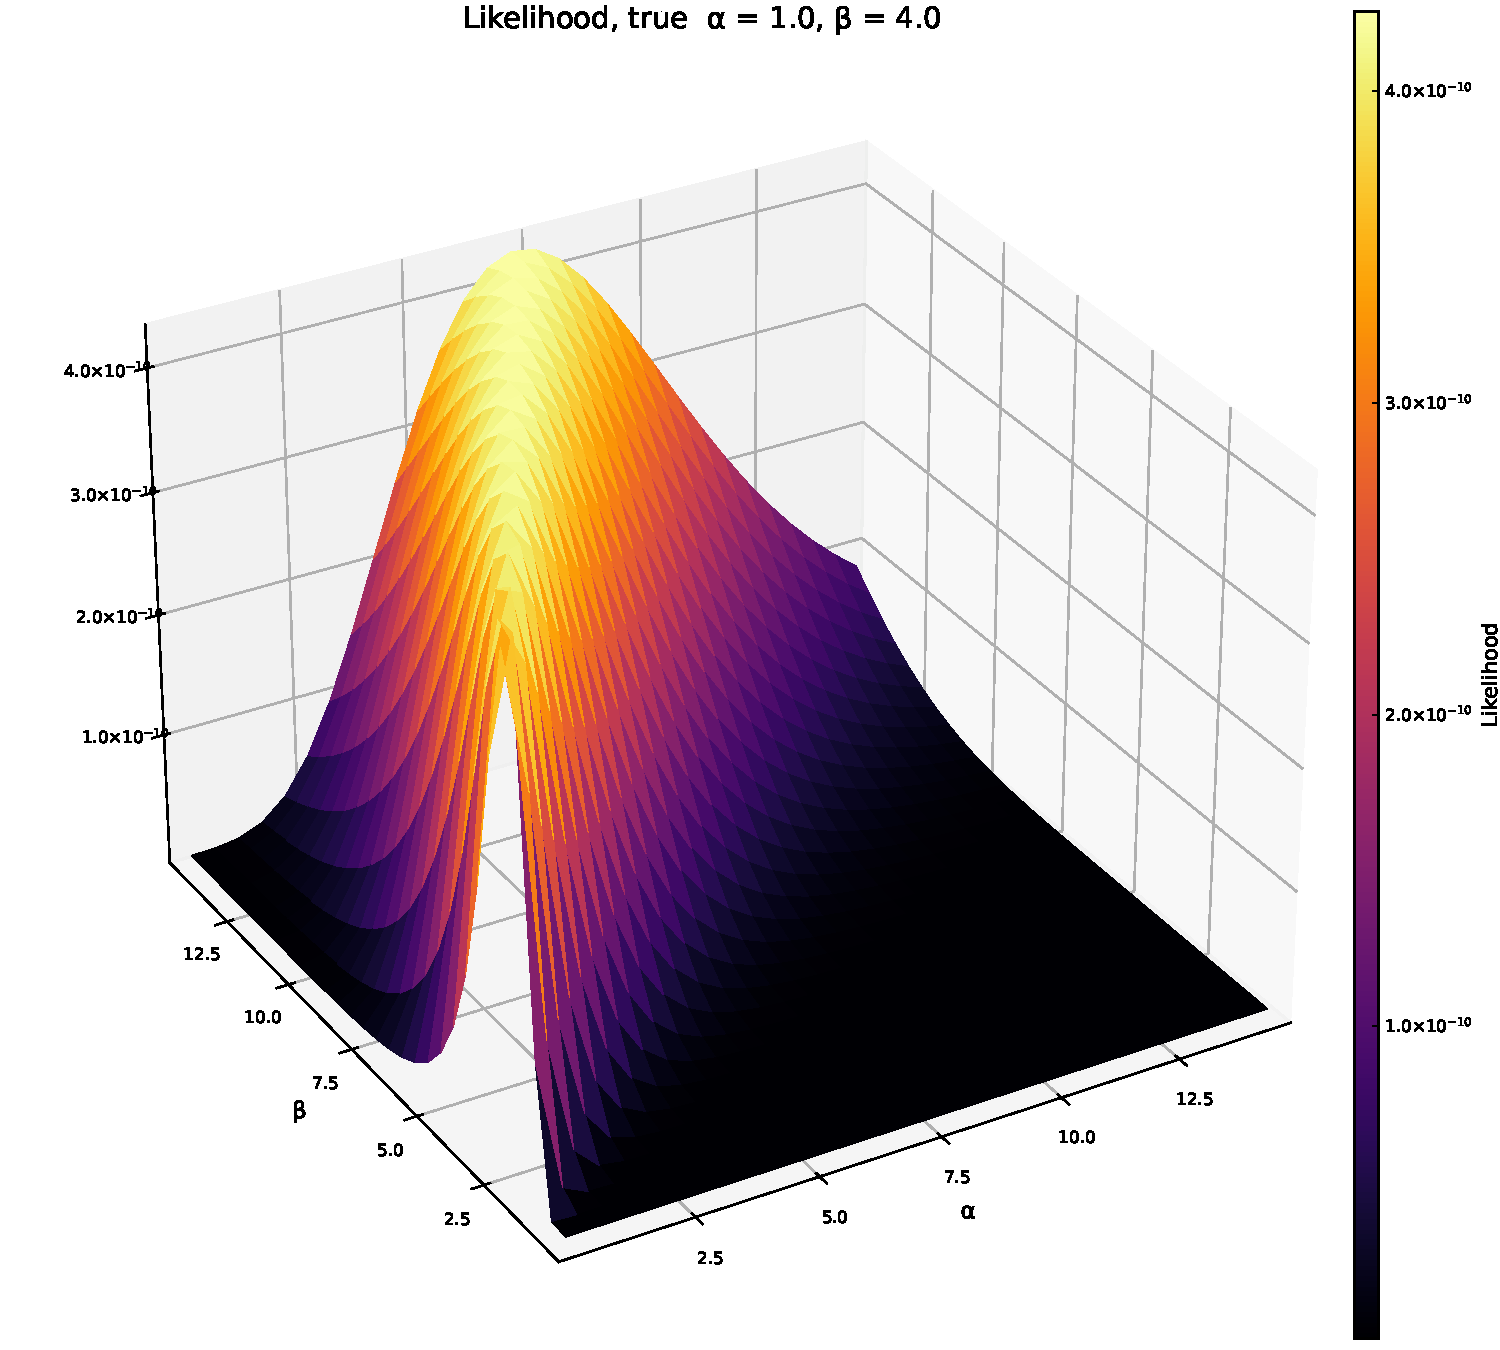
\includegraphics[width=0.9\textwidth]{../figures/Likelihood_sfplt_1.pdf} % first figure itself
    \end{minipage}\hfill
    \begin{minipage}{0.45\textwidth}
        \centering
        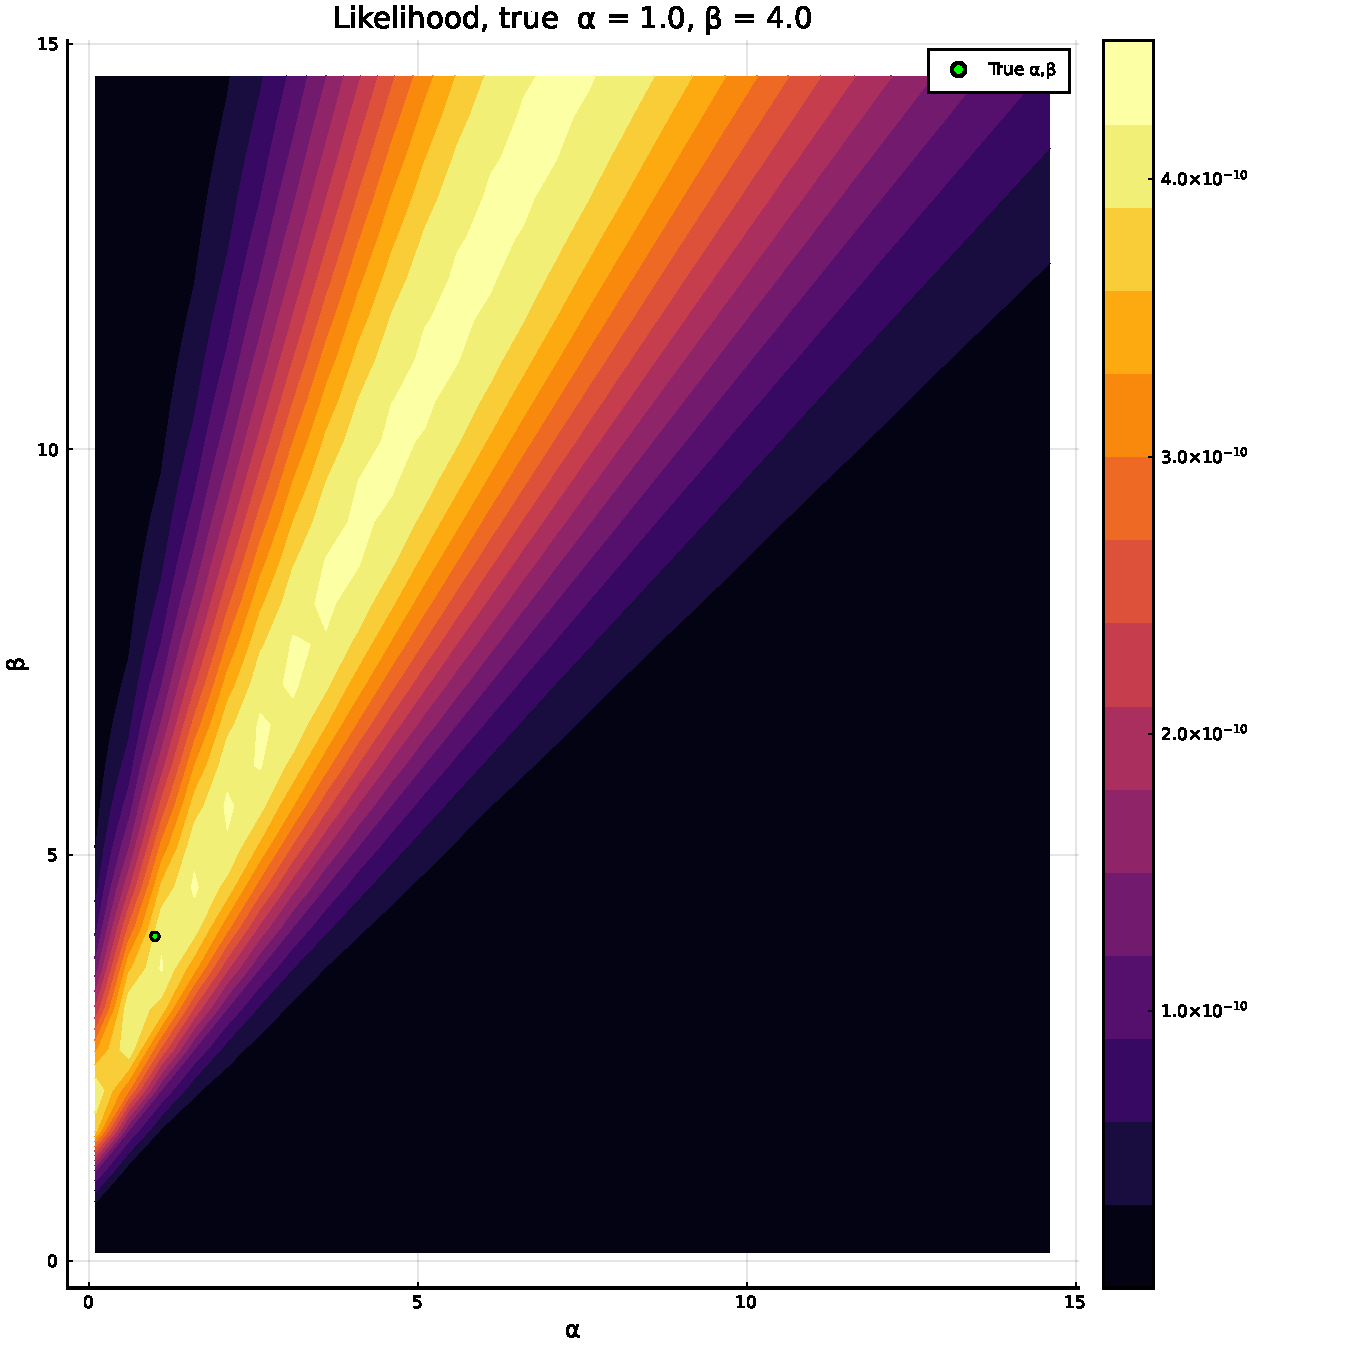
\includegraphics[width=0.9\textwidth]{../figures/Likelihood_contplt_1.pdf} % second figure itself
    \end{minipage}
    \caption{\small Likelihood function for data simulated by $\pi \sim Beta(1, 4), N = 100, n = 25, T = 2$}
\end{figure}

\begin{figure}
    \centering
    \begin{minipage}{0.55\textwidth}
        \centering
        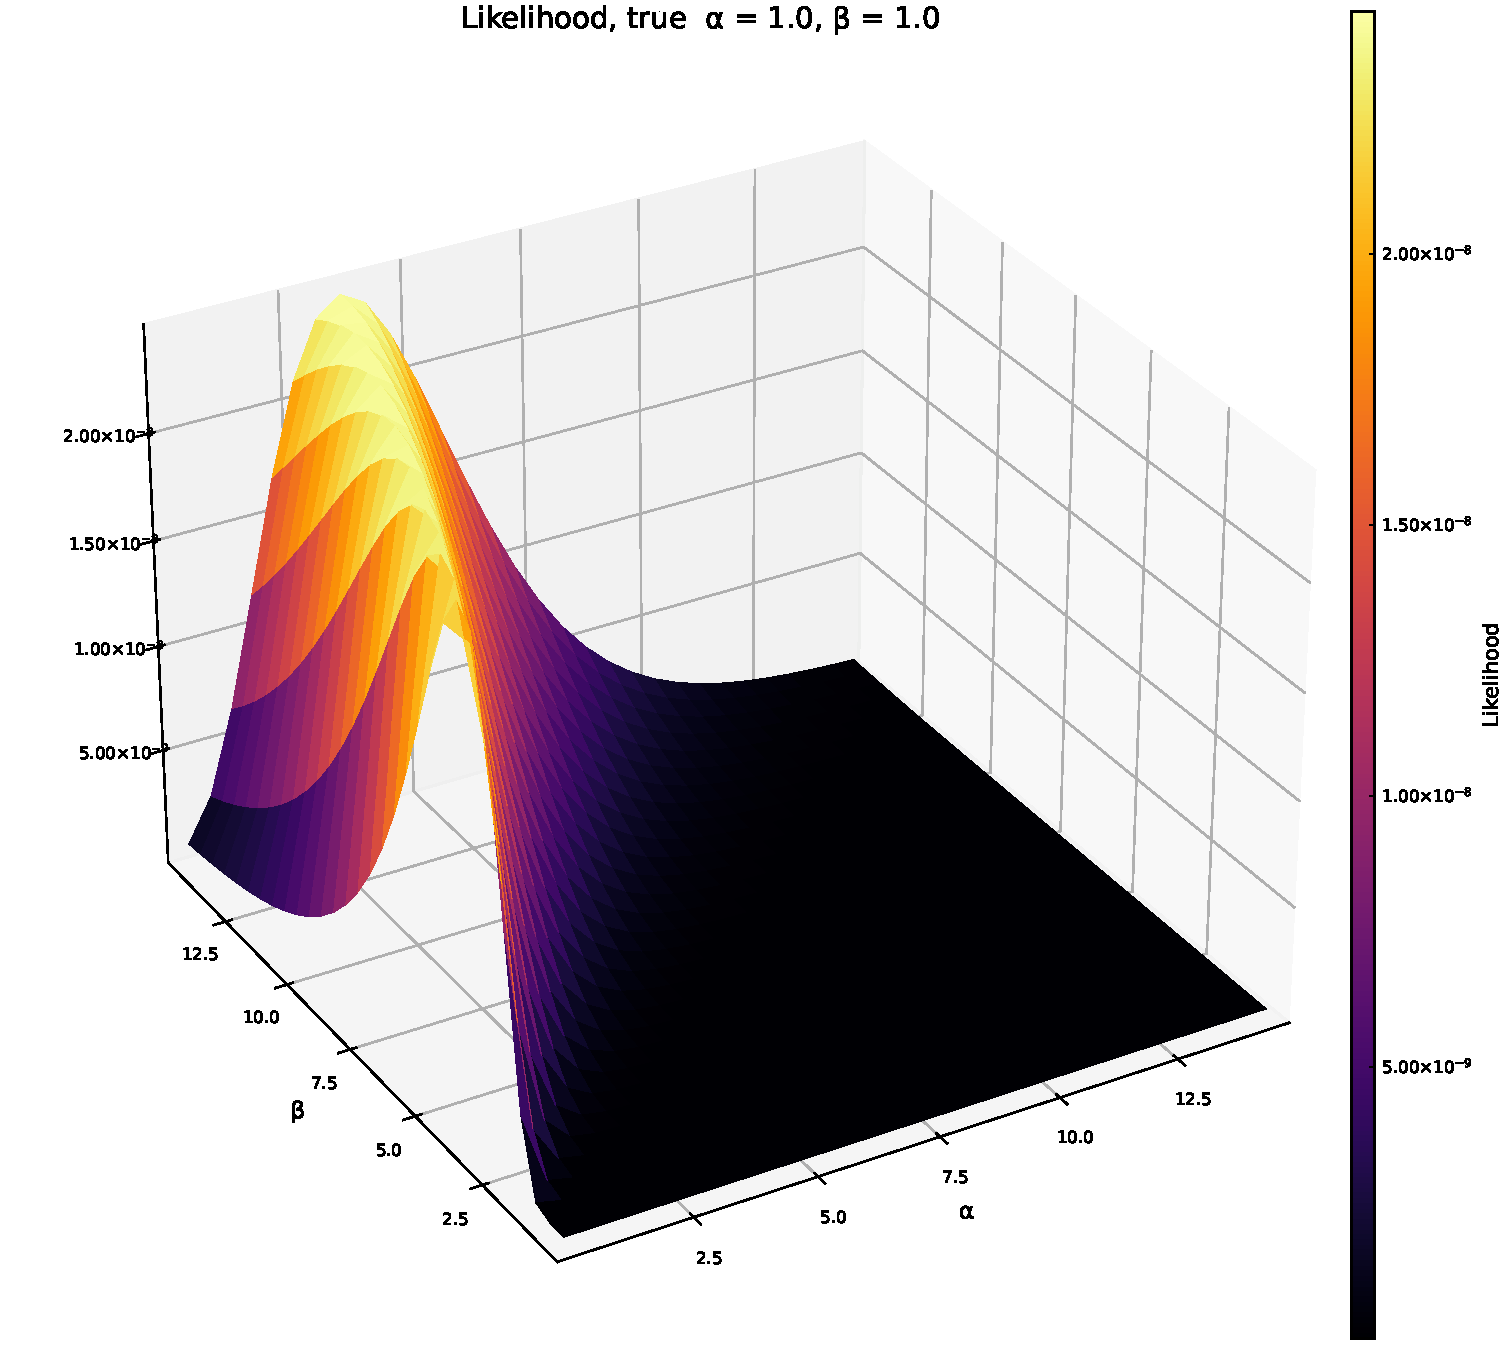
\includegraphics[width=0.9\textwidth]{../figures/Likelihood_sfplt_2.pdf} % first figure itself
    \end{minipage}\hfill
    \begin{minipage}{0.45\textwidth}
        \centering
        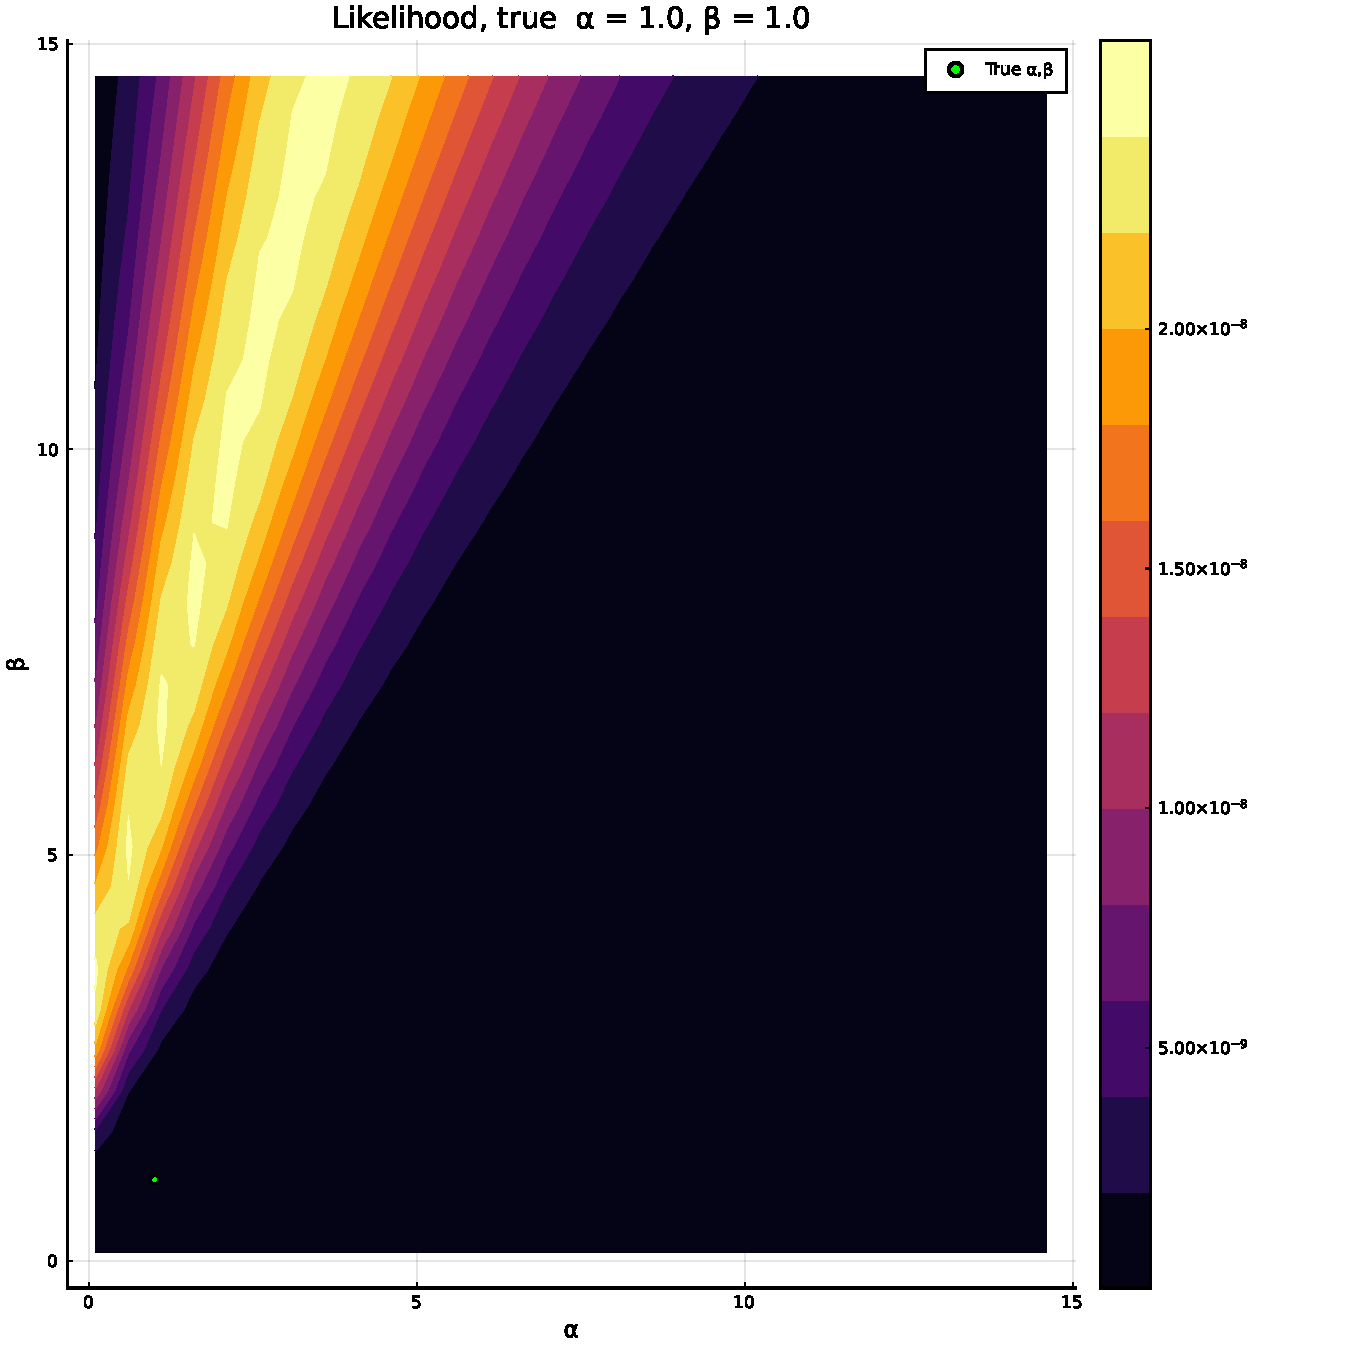
\includegraphics[width=0.9\textwidth]{../figures/Likelihood_contplt_2.pdf} % second figure itself
    \end{minipage}
    \caption{\small Likelihood function for data simulated by $\pi \sim Beta(1, 1), N = 100, n = 25, T = 2$}
\end{figure}

\begin{figure}
    \centering
    \begin{minipage}{0.55\textwidth}
        \centering
        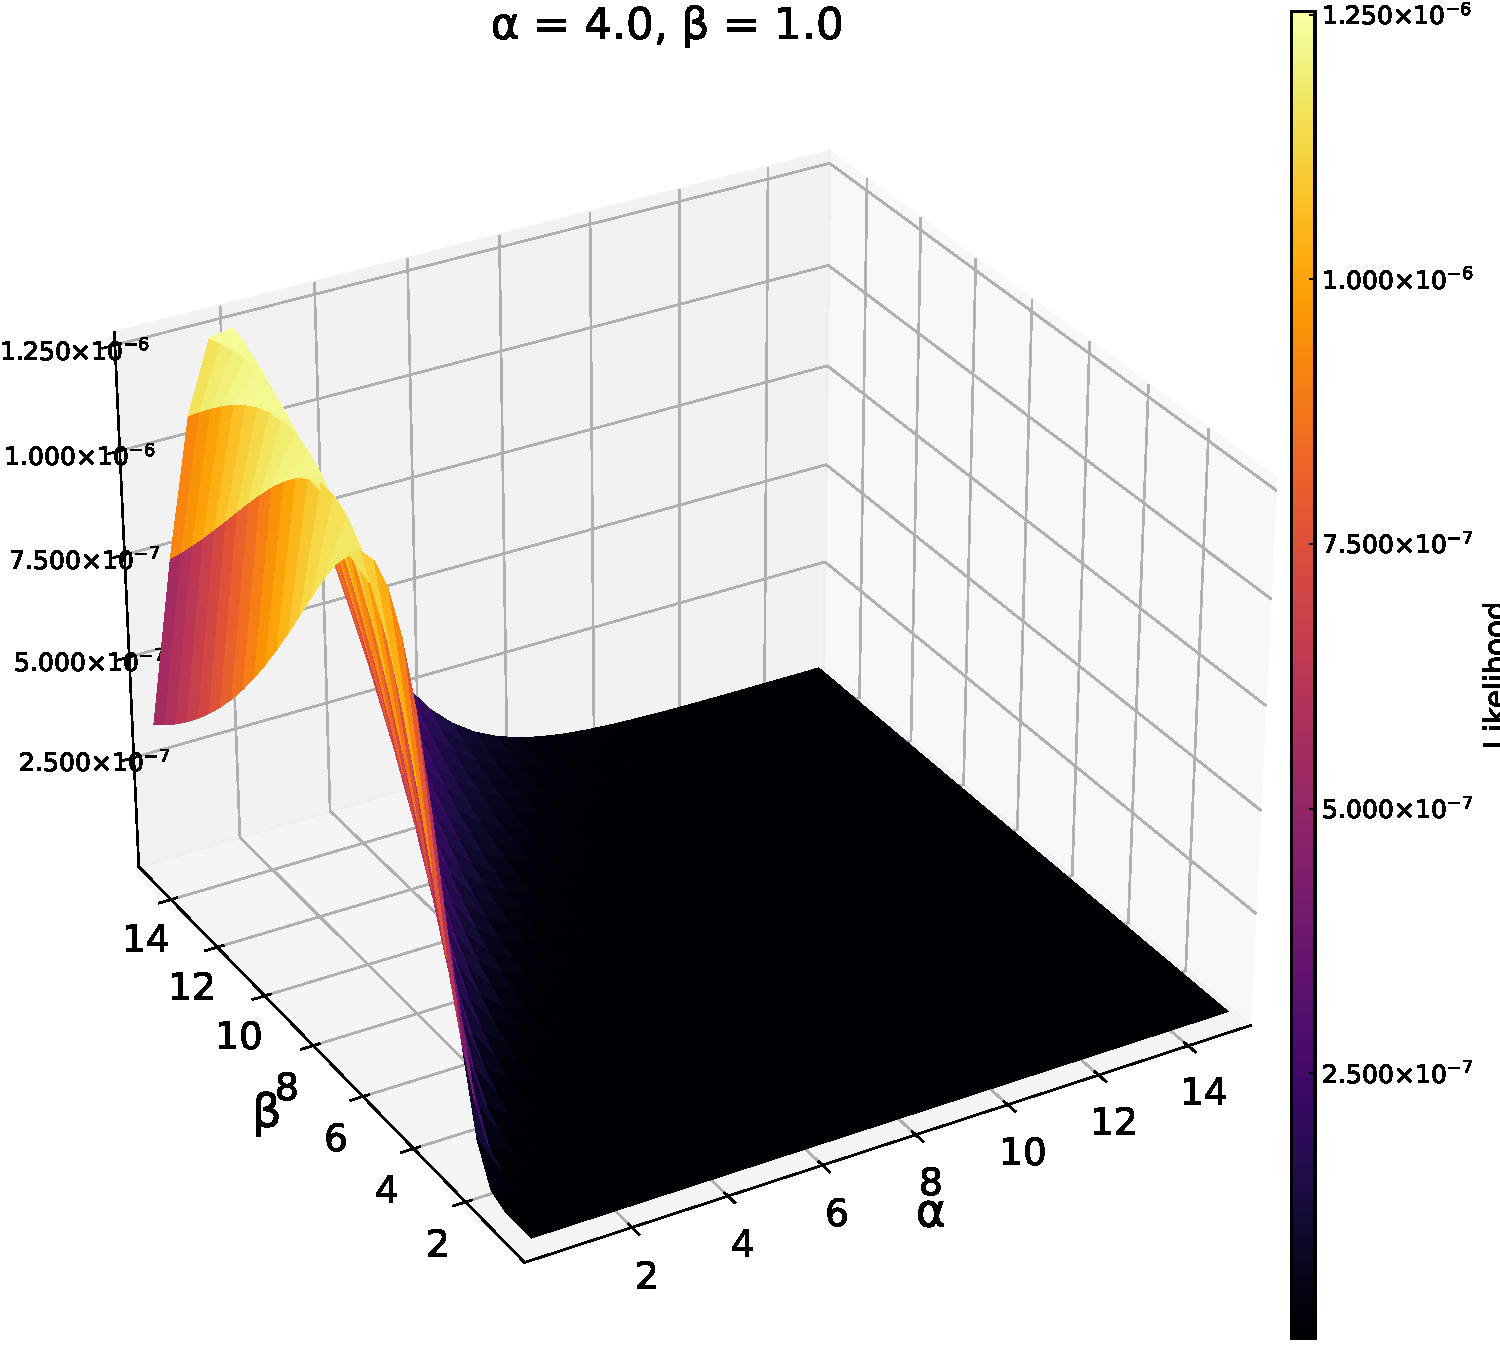
\includegraphics[width=0.9\textwidth]{../figures/Likelihood_sfplt_3.pdf} % first figure itself
    \end{minipage}\hfill
    \begin{minipage}{0.45\textwidth}
        \centering
        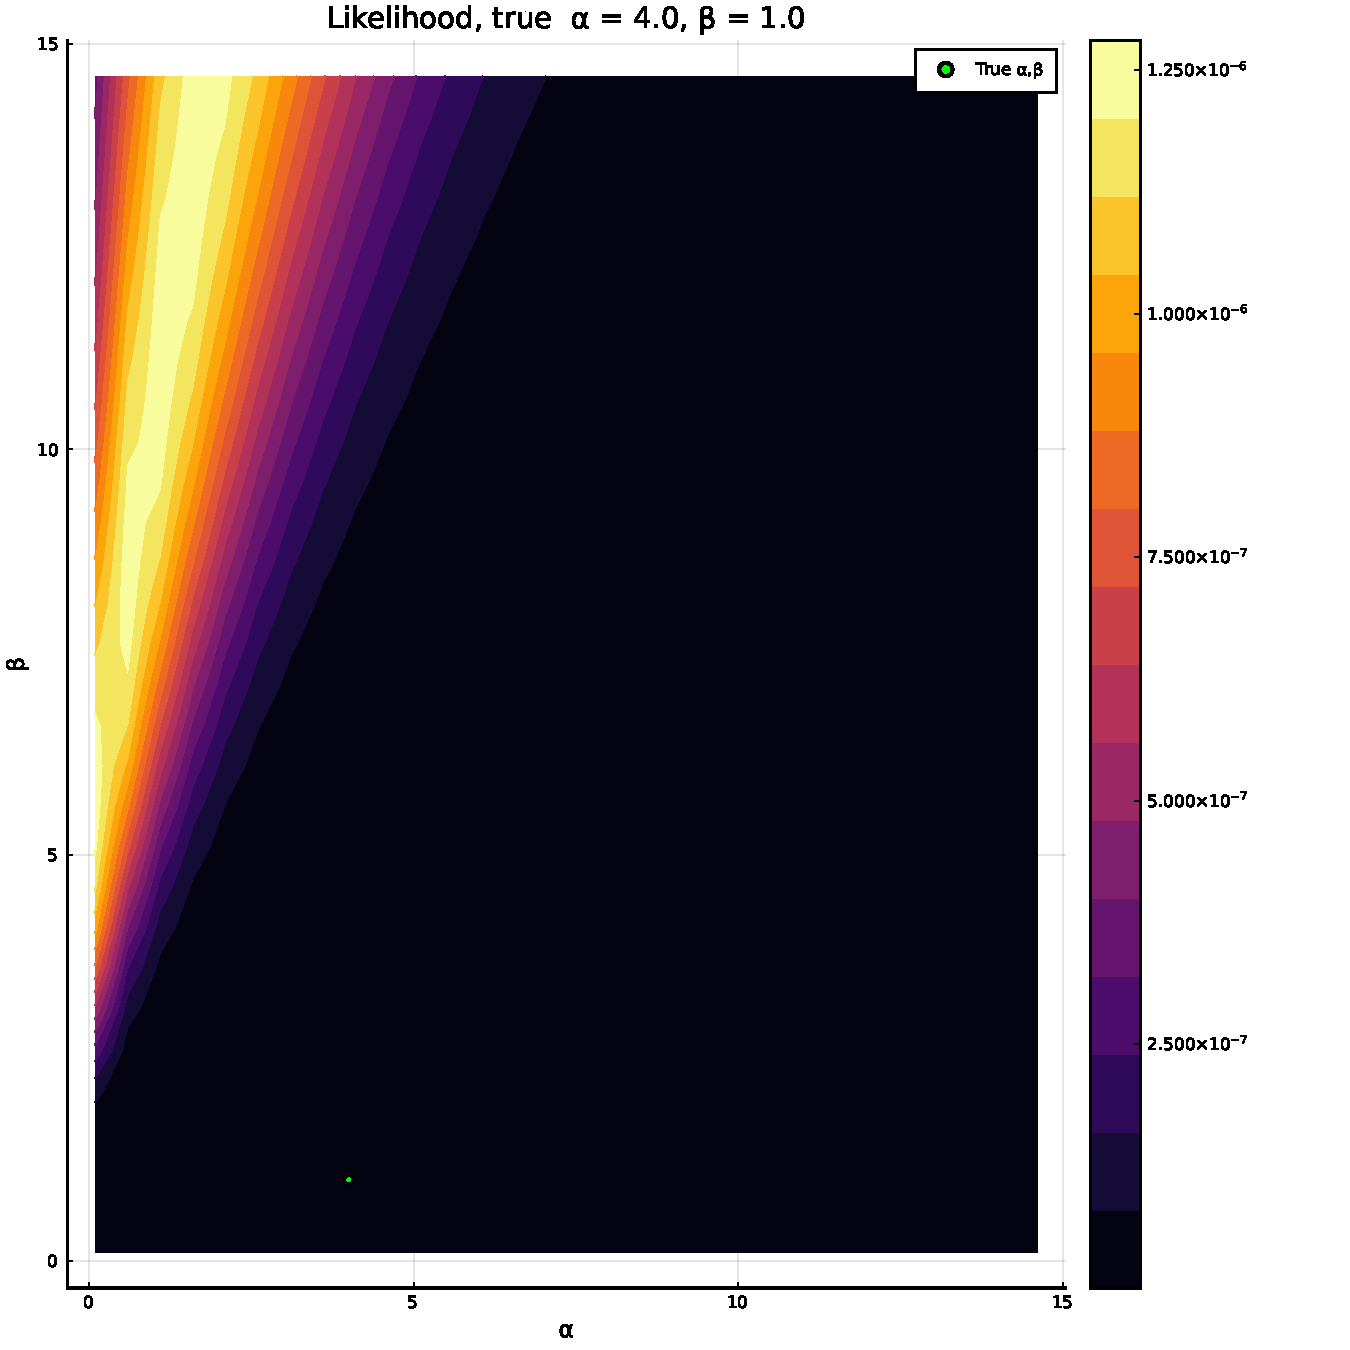
\includegraphics[width=0.9\textwidth]{../figures/Likelihood_contplt_3.pdf} % second figure itself
    \end{minipage}
    \caption{\small Likelihood function for data simulated by $\pi \sim Beta(4, 1), N = 100, n = 25, T = 2$}
\end{figure}

\end{document}
